\documentclass{article}
\usepackage{graphicx}
\usepackage{authblk}
\usepackage{amsfonts}
\usepackage{pifont}
\newcommand{\cmark}{\ding{51}}%
\newcommand{\xmark}{\ding{55}}%


\begin{document}

\title{Eagle: Making multiple-locus association mapping on a genome-wide scale routine}
\author[1]{Andrew W. George}
\author[1]{Arunas Verbyla}
\author[2]{Joshua Bowden}
\author[1]{Some other authors}

\affil[1]{Data61, CSIRO, Australia.}
\affil[2]{IM \&T, CSIRO, Australia.}

\maketitle






\begin{table}
\label{suptabsummary}
\caption{A summary of the features possessed by the Eagle package and the comparison implementations.}
\begin{tabular}{lccccccccc}
                                &  \multicolumn{9}{c}{Computer Software for Association Mapping} \\ \cline{2-10}
                                 & \multicolumn{6}{c}{Multiple-locus}  & & \multicolumn{2}{c}{Single-locus} \\  \cline{2-7}   \cline{9-10}
 Features                 & Eagle  & bigRR & glmnet & LMM-Lasso & MLMM & r2VIM     & & FaST-LMM & GEMMA \\  \hline
Purpose built$^1$    &   \cmark     &    \cmark      &  \xmark   &  \cmark  &  \cmark  &  \cmark && \cmark & \cmark           \\ [0.2cm]
Well documented$^2$           & \cmark &   \xmark   & \cmark   & \xmark     &   \cmark     & \xmark          && \cmark    &    \cmark    \\  [0.2cm]
Simultaneous   &    \cmark     &    \cmark        &   \cmark          &      \cmark             &  \xmark          &  \xmark              &&   \xmark   &  \xmark     \\  
fitting of SNPs     &         &            &             &                   &            &                &&      &      \\  [0.2cm]
Additional fixed effects$^3$          &   \cmark   &      \cmark      &     \cmark    &  \xmark                 &      \cmark      &      \cmark          &&      \cmark & \cmark     \\   [0.2cm]
Data larger than RAM$^4$                   &   \cmark    &      \xmark      & \xmark          &  \xmark    &  \xmark    &   \xmark     && \cmark      & \xmark    \\  [0.2cm]
Threshold free$^5$        &    \cmark     &  \xmark    &  \xmark         &    \xmark               &     \cmark       &  \xmark              &&  \xmark   & \xmark      \\  [0.2cm]
Informative error checking           &  \cmark      &     \xmark        &      \xmark     &           \xmark        &      \xmark       &         \xmark       && \cmark  & \xmark \\ \hline

\end{tabular}
{$^1$ \scriptsize{Computer software specifically designed for the analysis of data from GWAS.}}\\
{$^2$ \scriptsize{More than just a readme file or comments in an example file. Those programs with ticks had detailed user manuals.}}\\
{$^3$ \scriptsize{Ability to accommodate additional fixed effects in the model such as age, sex, and population structure effects.}} \\
{$^4$ \scriptsize{Able to deal with data larger than the memory capacity of the computer.}} \\
{$^5$ \scriptsize{Results reported as the set of SNP closest to the genes influencing a trait. No need to construct thresholds to determine 
significance of the findings.}}\\
{$^6$  \scriptsize{All the programs terminated on errors. However, not all the programs informed the user of the cause and how to fix the errors.}}\\
\end{table}






\begin{figure}
\caption{Memory usage (in gigabytes) of Eagle and the other association mapping programs across 
the six simulation scenarios. The maximum amount of memory on the computer is 128 gigabytes. 
The x-axis is on the log scale. GEMMA, a single-locus implementation, had the lowest memory usage. 
Of the multiple-locus implementations, Eagle had the lowest memory usage. Also, it 
was the only multiple-locus 
implementation able to produce results for data under  scenario 10000 x 1.5M. This is due to its ability 
to handle data larger than the available memory of a computer. FaST-LMM was run where all the SNP data are used 
to estimate the relationship matrix (FaST-LMM$^{all}$)   and where genotype data from every five-hundredth SNP are used to 
estimate the relationship matrix (FaST-LMM$^{few}$)}.
\begin{center}
\includegraphics[width=15cm, height=15cm]{mem.eps}
\end{center}
\end{figure}


\begin{table}
\caption{The median run times (in minutes) of Eagle and the other association mapping programs across the six simulation scenarios. }
\begin{tabular}{llcccccc}
              &           &  \multicolumn{6}{c}{Simulation Scenarios} \\ \cline{3-8}
 Method & Name & 150 x 5K & 1500 x 50K & 350 x 400K & 2000 x 500K & 4000 x 1.5M & 10000 x 1.5M \\ \hline
  Multiple & Eagle 	&	   0.08  &   1.62   &  \bf{2.7}1  &   \bf{13.65}   & \bf{127.63}  &   699.55  \\
               & MLMM 	&	   0.15    &  2.91    & 19.04  &  143.01  &  870.84  &     \\
               & glmnet 	&	  0.11     & 3.95    & 14.06    & 74.03    &        &    \\
               & r2VIM 	&	   0.09    &  3.66    &  5.51    & 50.59    & 380.52  &   \\ 
               & bigRR 	&	    1.01   & 113.35   &  54.99   & 1030.61  &        &     \\
               & LMM-Lasso 	&     0.57  &   52.08 &    92.20  & 1031.85 &           &     \\ \\
Single     &  GEMMA 	&      0.02  &   5.02   &   6.17  &   84.83   & 723.33  & 4071.60 \\
               & FaST-LMM$^{few}$ 	&    \bf{0.01}   &  \bf{0.80}   &   7.07   &  20.16   & 193.90   & \bf{346.19} \\ 
               & FaST-LMM$^{all}$   	&   0.03   & 2.96  &    7.90   &  41.27  &            &   \\ \hline
\end{tabular}

\end{table}


\end{document}
